\documentclass[12pt,a4paper]{article}

% Margins.
\setlength{\oddsidemargin}{0in}
\setlength{\evensidemargin}{0in}
\setlength{\headheight}{12pt}
\setlength{\headsep}{42pt}
\setlength{\topmargin}{-54pt}
\setlength{\textwidth}{6.5in}
\setlength{\textheight}{10in}

\usepackage{amsmath}
\usepackage{float}
\usepackage{graphicx}
\usepackage[hyphens]{url}
\usepackage{hyperref}	% Clickable links to figures, references and urls.

% Drawing.
\usepackage{pgf}
\usepackage{tikz}

% Listings for formatting code.
\usepackage{listings}
\usepackage{textcomp}
% General options.
\lstset{breaklines=true, basicstyle=\small\ttfamily, tabsize=4, numbers=none, stepnumber=1, frame=none, showstringspaces=false, upquote=true}
% C++ specific high-lighting. Comments are 50/50 shades of green/black and strings coloured with 60/40 red/black mixture.
\lstset{language=[ISO]C++, commentstyle=\color{green!50!black}, keywordstyle=\color{blue}, stringstyle=\color{red!60!black}}

%opening
\title{\vspace{-2cm}Programming for Engineers I\\Class 12\\Sessional Exam 01 Discussion}
\author{Attique Dawood}

% Marks of each question.
\def\QOne{5}
\def\Qtwo{10}
\def\Qthree{20}
\def\Qfour{15}
\def\Qfive{30}
\def\Qsix{20}
\def\TotalMarks{100}

\begin{document}
\maketitle
\section{Announcements}
\begin{itemize}
\item None.
\end{itemize}
\section{Revision}
\begin{itemize}
\item \verb|switch|
\end{itemize}
% For solution every line is worth 0.5 cm in the box.
\section{Exam Solution}
\noindent\textbf{Question 1: Simple Output\hfill \QOne~marks}\\
Write the output of following code snippet.
\begin{lstlisting}
#include <iostream>
using namespace std;

int main()
{
	int x = 3;
	char c = '3';
	cout << "x is " << x << " and c is " << c << endl;
	
	return 0;
}
\end{lstlisting}
\begin{figure}[H]
\begin{lstlisting}
 x is 3 and c is 3
\end{lstlisting}
\vspace{-1cm}
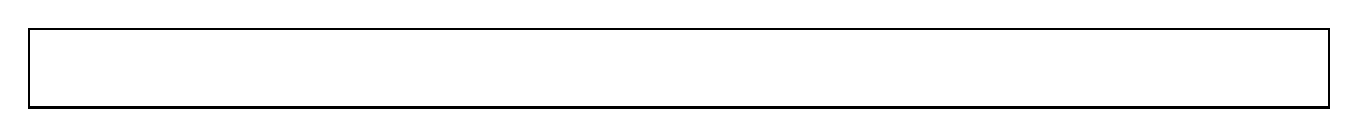
\begin{tikzpicture}
	\draw[thick] (0cm,0cm) rectangle (\textwidth, 1cm);
\end{tikzpicture}
\end{figure}

\noindent\textbf{Question 2: Compilation Steps \hfill \Qtwo~marks}\\
What are the different steps involved in programming cycle (from editing to creation of executable)? 
\begin{figure}[H]
\begin{lstlisting}
 1. Coding.
 2. Preprocess.
 3. Compile (.obj)
 4. Link (.exe)
 5. Execute.
 6. Debug.
\end{lstlisting}
\vspace{-3.25cm}
\begin{tikzpicture}
	\draw[thick] (0cm,0cm) rectangle (\textwidth, 3cm);
\end{tikzpicture}
\end{figure}

\noindent\textbf{Question 3: Bitwise and Shift Operators \hfill $4\times 5=$\Qthree~marks}\\
Assume 4 bit unsigned binary numbers. Evaluate the following:
\begin{enumerate}
\item \verb|4 & 5|
\item \verb$4 | 7$
\item \verb|3 ^ 9|
\item \verb|7 >> 2|
\item \verb|8 << 1|
\end{enumerate}
\begin{figure}[H]
\begin{lstlisting}
 1. 4 & 5 = 0100 AND 0101 = 0100 or 4
 2. 4 | 7 = 0100 OR 0111 = 0111 or 7
 3. 3 ^ 9 = 0011 XOR 1001 = 1010 or 10
 4. 7 >> 2 = 0111 >> 2 = 0001 or 1
 5. 8 << 1 = 1000 << 1 = 0000 or 0
\end{lstlisting}
\vspace{-2.75cm}
\begin{tikzpicture}
	\draw[thick] (0cm,0cm) rectangle (\textwidth, 2.5cm);
\end{tikzpicture}
\end{figure}

\noindent\textbf{Question 4: Signed Integers \hfill \Qfour~marks}\\
Assuming 16 bit signed integer, what is the bit representation of -147? Show how this number is stored in computer memory.
\begin{figure}[H]
\begin{lstlisting}
 147 = 128 + 16 + 3
     = 2^8 + 2^4 + 3
     = 100000000 + 10000 + 11
     = 10010011 = 1001 0011
 147 as 16 bit unsigned integer = 0000 0000 1001 0011
 
 -147 = 2's complement of 147 = 1111 1111 0110 1100 + 1
                              = 1111 1111 0110 1101
                              = FF 6D
                              
  Memory Storage: 6D FF
\end{lstlisting}
\vspace{-5.75cm}
\begin{tikzpicture}
	\draw[thick] (0cm,0cm) rectangle (\textwidth, 5.5cm);
\end{tikzpicture}
\end{figure}

\newpage
\noindent\textbf{Question 5: Float Representation \hfill $15+15=$\Qfive~marks}\\
a. Convert 37.390625 to 32 bit floating point representation. Also show how this number is stored in computer memory.
\begin{figure}[H]
\begin{tikzpicture}
	\draw[thick] (0cm,0cm) rectangle (\textwidth, 10cm);
\end{tikzpicture}
\end{figure}
\noindent b. Convert the following 32 bit floating point number into decimal.\\
\verb|1 10000110 10110110000000000000000|
\begin{figure}[H]
\begin{tikzpicture}
	\draw[thick] (0cm,0cm) rectangle (\textwidth, 8cm);
\end{tikzpicture}
\end{figure}
\newpage
\noindent\textbf{Question 6: Loops \hfill \Qsix~marks}\\
Write C++ code to input an integer from user and determine if it is a prime number.
\begin{figure}[H]
\begin{tikzpicture}
	\draw[thick] (0cm,0cm) rectangle (\textwidth, 12cm);
\end{tikzpicture}
\end{figure}
\end{document}